\chapter{Basic circuit theory}
Electrical circuits are fundamental building blocks in, more or less, every electronic device you can think of. The simple act of flipping a switch, e.g. to turn on the light, completes an electrical circuit. The purpose of the circuit is to carry electrical current, either in an open or closed circuit. The electrical components in a circuit are typically resistors, capacitors,  switches, and an electrical 	source (a battery, for instance).
\\ 
In this chapter, if a function is assumed constant, it is denoted with capitalization of its original notation. 
\\ 
\\
The different elements of the circuit can be divided into two categories: active and passive. Active elements supply energy to the system, e.g. a battery, whereas passive elements absorb energy, e.g. a light bulb. A circuit with a battery and a bulb can be represented in the following way.
\begin{figure}[H]
\begin{center}
\begin{circuitikz}[american voltages]
\draw
to[battery, battery1=$V_{B}$, color=blue] (0,2)

to[short, -] (2,2)
[short](2,2)

[short] (2,2)
to [lamp, l=$R_{\text{bulb}}$, color=green](2,0)

(0,0) to [short] (2,0);
\end{circuitikz}
\end{center}
\caption{A circuit with a battery and a light bulb}
\label{fig:bulb}
\end{figure} 
In figure \ref{fig:bulb} the active element is a battery, and the passive element is a light bulb. Charge is transported by the current from the positive terminal of the battery, through to the light bulb. The light bulb absorbs the energy from the charge, which is then transported to the negative terminal of the battery.
\\
\section{Current}
Current is the force that moves charge through a circuit. Current can be defined as an amount of charge moved over a time interval. This can be expressed as the following relation:
\begin{align}
i(t)=\dfrac{dq(t)}{dt} \Leftrightarrow q(t)=\int_{0}^{t}i(x)dx,
\end{align}
where $i(t)$ is the current (in ampere, $A$), to a given time $t$ (in seconds, $s$), and $q(t)$ is the function for charge at a given time $t$. $q(t)$ is measured in Coulomb$(C)$.
\\
There exists two types of current, alternating current (AC) and direct current (DC). DC current is constant, while AC alternates, see figure \ref{fig:ACDC}. 
\begin{figure}[H] 
\begin{tikzpicture}
\begin{axis}[ticks=none,
axis lines =center,
xlabel={t},
ylabel={i(t)},
    height=7cm, width=9cm,
    xmin=0, xmax=10, ymin=-2, ymax=2]
\addplot [
    domain=0:10, 
    samples=100, 
    color=red,
]
{1};
\addlegendentry{$DC$}
\addplot [
    domain=0:10, 
    samples=100, 
    color=blue,
    ]
    {sin(\x r)};
\addlegendentry{$AC$}
\end{axis}
\end{tikzpicture}
\caption{Current for AC and DC versus time}
\label{fig:ACDC}
\end{figure}
\section{Voltage}
Voltage ($V$), also called electric potential difference, is the change in potential energy a charge undergoes, when it passes through two given points in a circuit. This is expressed in the following equation:
\begin{align}
	V=\dfrac{dU(q)}{dq},
\end{align}
\\
where $U(q)$ (in joules, $J$) is the function for potential energy, given a charge $q$.
\section{Resistor}
When a resistor, which is a passive element, is added to the circuit, it creates a resistance ($\Omega$). Resistance makes it more difficult for the current to pass through the element. Resistance is defined as the proportional constant between current and voltage. The mathematical relation of this is given by:
\begin{align} 
\label{Ohm}
v(t)=R\cdot i(t),  R\geq0,
\end{align}
where $R$ is resistance (in Ohm, $\Omega$).
\section{Capacitor}
A capacitor is a passive element of a circuit. A capacitor consists of two similar sized plates. When a voltage is applied to the circuit, the capacitor gets charged. The capacitance is the amount of energy a capacitor can store, when it is fully charged. The capacitor gets charged when positive a charge is transferred from one plate, through the circuit, to the other plate. The capacitance is given by the following equation:
\begin{align*}
C=\dfrac{\epsilon_{0}A}{d},
\end{align*}
where $C$ is the capacitance (in farad, $F$), $\epsilon_{0}$ is the permittivity of free space, which is equal to $8.85 \cdot 10^{-12}                                                 \frac{F}{m}$. $A$ is the surface area of the plates (in square meters, $m^{2}$), and $d$ is the distance between the two plates (in meters, $m$).
\\
The charge of a capacitor across a voltage ($V$) and capacitance of ($C$) is equal to:
\begin{align}
\label{QCV}
Q=CV	
\end{align}
\section{Circuit diagrams}
Electrical circuits are visually represented in circuit diagrams. In addition to the above-mentioned elements, the circuit diagrams introduce three terms: nodes, branches, and loops. Elements are \textit{branches} i.e.  the voltage supply, resistors, capacitors, and the like. \textit{Nodes} connect the \textit{branches} of the circuit. Lastly, any closed path in the circuit, in which no node is encountered more than than once, is called a \textit{loop} \cite[page~32]{bcircuit}. An example of a circuit is shown below.

\begin{figure}[H]
 \begin{center}
\begin{circuitikz}[american voltages]
\draw
to[battery, battery1=$V_{B}$, color=blue] (0,2)
to[resistor, R=$R_1$, color=red] (2,2)
to[resistor, R=$R_2$, color=red] (2,0)
to[short, -] (0,0)
[short, -](2,2) to [short, -] (3,2)
to[resistor, R=$R_3$, color=red](3,0)
to[short, -] (2,0)
[short](3,2) to [short] (5,2)
to [C=$C$, color=green](5,0)
to [short, -] (3,0)
(0,0) to [short, l_=$N_3$, -] (5,0)
(2,2) to [short, l^=$N_2$, -] (5,2)
(0,1) to [short, l^=$N_1$, -] (0,2);
\end{circuitikz}
\end{center}
 \caption{A circuit with a battery, three resistors and a light bulb}
\end{figure}

This circuit has five branches, which are shown marked in color: a battery (in blue), three resistors ($R_1, R_2,$ and $R_3$, in red), and the light bulb (in green). The three nodes of the circuit ($N_1$, $N_2$, and $N_3$) connect the branches. Additionally, there are three loops, all of which have the same starting and ending point, $V_{battery}$. The first loop passes through $R_2$ and $R_1$, and returns to the starting point. Similarly, the second loop passes through $R_3$ and $R_1$, and returns. The third, and final, loop runs through the light bulb, then $R_1$, and returns. 

\subsection{Kirchhoff's Laws}
\textbf{Kirchhoff's Current Law (KCL)}
\\
Observe a circuit up until a node, past which the path of the circuit splits in two. The current encountering the node does not accumulate (as it would e.g. in a battery). Instead, all electrons flowing to that node split up between the available paths, and continue to flow through the circuit. This is Kirchhoff’s current law (KCL), which states that the algebraic sum of all currents in a node is equal to zero. 
\begin{align}
\sum_{j=1}^{N} i_{j}(t) = 0,
\end{align}
where $i_{j}(t)$ is the $j$'th current entering the node through branch $j$, with $N$ branches connected to the node. \cite[page~32]{bcircuit}
\\
\\
\textbf{Kirchoff's Voltage Law (KVL)}
\\
KVL states: In a circuit, the algebraic sum of all voltages in a loop is equal to zero. This can be expressed mathematically  as,
\begin{align}
\sum_{j=1}^{N} v_{j}(t) = 0,
\end{align}
where $v_{j}(t)$ is the voltage in the $j$'th voltage with $N$ voltages.\citep[page~34]{bcircuit}\\

\section{RC Circuit}
An RC circuit is an electrical circuit consisting of resistors and capacitors. In its simplest form, it is composed of one of each. In that case, a charged capacitor placed in series with a resistor will discharge back through the resistor \cite[p~21]{artof}. 

\begin{figure}[H]
 \begin{center}
\begin{circuitikz}[american voltages]
\draw (0,0)
to[sqV, sqV=$v_{input}$] (0,2)
to (6,2)
to[short, -] (4,2)
to[C=$C$] (4,0)
to (6,0)
to (4,0)
to [resistor, R=$R$] (0,0);
\draw [>=latex', <->] (6,1.75) -- node[anchor=west] {$v_{C}(t)$} (6,0.25);
\end{circuitikz}
\end{center}
 \caption{An RC circuit with a capacitor and a resistor}
\end{figure}

If the voltage in (3.4) is replaced with a change in voltage, with respect to time: $\dfrac{dv}{dt}$, the right side of (3.4) becomes: $C\dfrac{dv}{dt}$. This change in voltage will result in a change in charge, with respect to time. Since current is a change in charge, (3.4) can be rewritten as:
\begin{align}\label{I_C}
I_{C}= C \dfrac{dv}{dt}
\end{align}
\subsection{Transient analysis}
\label{sec371}
To find out how the voltage of a capacitor changes over time when it is charged and discharged, transient analysis is used.
\\
Kirchhoff's Current Law states that the sum of the currents in a node is equal to zero. In the case of an RC-circuit, the law can be written as the following equation:
\begin{align*}
I_{C}+I_{R}=0 \Leftrightarrow 
I_{C}= -I_{R}
\end{align*}
Inserting the definition of the current through the capacitor \eqref{I_C} and the resistor \eqref{Ohm} yields a differential equation, which can then be separated as stated in subsection \ref{SDE}:
\begin{align*}
C \dfrac{dv}{dt}&=\dfrac{-V}{R} \\
\dfrac{dv}{dt} &= -V\dfrac{1}{RC} \\
\end{align*}
The equation is now in the same form as \eqref{SDE}, in which it can be solved as following:
\begin{align}
\int \dfrac{1}{V}dv =& \dfrac{-1}{RC} \int dt\nonumber \\
\ln(V) =& \dfrac{-t}{RC} + A \nonumber\\
V =& e^{\frac{-t}{RC}}e^{A}\label{V_eA}
\end{align}
Since $A$ is the constant of integration, the constant $e^A$ can be defined as a new constant $e^A=B$.
\\
By definition, the starting voltage of the capacitor is given by $V_C(t=0)=V_0$; inserting this and $B$ into \eqref{V_eA} yields the following equation: 
\begin{align}
V(t)= e^{\frac{-t}{RC}}B \label{V_eB}\\
V(0)= B = V_0\nonumber
\end{align}
The constant $B$ is then equal to the starting voltage $V_0$. By inserting this into \eqref{V_eB}, the final function is found:
\begin{align}
\label{V_down}
\Aboxed{
 V(t) = V_0e^{\frac{-t}{RC}}
 }
\end{align}
The function in \eqref{V_down} describes how the voltage decreases over time, when the capacitor is discharged.
\\
\\
Now the function for when the capacitor charges is derived. KVL states that the sum of the voltages over a loop must be equal to zero. 
\\
In an RC circuit with a battery this can be written algebraic as:
\begin{align*}
V_B-V_R-V_C =& 0 \\
V_B=&V_R+V_C
\end{align*}
$V_R$ and $V_C$ have negative signs, since their elements create a negative potential difference when charge passes through them.
\\
By Ohm's law, the voltage of the resistor can be expressed as $V_R=IR$. By definition \eqref{QCV} the voltage of the capacitor can be expressed as $V_C=\dfrac{Q}{C}$. This is inserted in the equation above:
\begin{align*}
V_B=&V_R+V_C \\
V_B =& IR+\dfrac{Q}{C}
\end{align*}
As stated earlier, current is defined as $I =\dfrac{dq}{dt}$, this is inserted in place of $I$. Both sides are also divided by $R$:
\begin{align*}
\dfrac{V_B}{R} &= \dfrac{dq}{dt} + Q\dfrac{1}{RC} \\
\end{align*}
This is a linear differential equation of the first order in the form of \eqref{FODE_form}:
\begin{align*}
\dfrac{dy}{dx}&=\dfrac{dq}{dt}
\\
h(x)&=\dfrac{1}{RC}
\\
H(x)&=\int \dfrac{1}{RC}=\dfrac{t}{RC}
\\
y &= Q
\\
g(x)&= \dfrac{V_B}{R}
\end{align*}
This is inserted in the general solution \eqref{FODE_solution}:
\begin{align}
Q&= e^{\frac{-t}{RC}}\int_{0}^{t}e^{\frac{t}{RC}}\dfrac{V_B}{R}dt
\\
Q&= e^{\frac{-t}{RC}}\dfrac{V_B}{R}\int_{0}^{t}e^{\frac{t}{RC}}dt \label{Q_1}
\end{align}
The integral is now solved by substitution. First $u$ and $\dfrac{du}{dt}$ are defined:
\begin{align*}
u &= \dfrac{t}{RC}
\\
\dfrac{du}{dt}&=\dfrac{1}{RC}
\\
dt &=RC du
\end{align*} 
By inserting these definitions into \eqref{Q_1} the equation looks like this:
\begin{align*}
Q&=e^{\frac{-t}{RC}}\dfrac{V_B}{R}\int_{0}^{\frac{t}{RC}}e^u du
\\
Q&=e^{\frac{-t}{RC}}\dfrac{V_B}{R}[e^u]_{0}^{\frac{t}{RC}}
\\
Q&=V_B C e^{\frac{-t}{RC}}(e^{\frac{t}{RC}}-1)
\\
Q&=V_B C (1-e^{\frac{-t}{RC}})
\end{align*} 
The voltage of a capacitor is given as $V_C=\dfrac{Q}{C}$. By dividing the equation above with $C$, the function for charging a capacitor is found.
\begin{align}
\label{V_up}
\Aboxed{
V_C(t)=V_B(1-e^{\frac{-t}{RC}})
}
\end{align}
\subsection{RC circuit experiment}
In the following section an RC circuit experiment has been made. Data from an RC circuit will be compared to values from a mathematical model.
\subsection{Theoretical values}
The resistor and capacitor in the experiment, had the following values:
\begin{align*}
 R =& 4770\Omega \\
 C =& 97.61nF
\end{align*}
The circuit was set up as follows:
\begin{figure}[H]
	\begin{center}
\begin{circuitikz}[american voltages]
\draw
to[sqV, sqV=$1 V$] (0,2)
to[resistor, R=$4770 \Omega$] (4.5,2)

[short](3,2) to [short] (5,2)

to [short, C=$97.61 nF$] (5,0)
(0,0) to [short, -] (5,0)

(0,1) to [short, -] (0,2);
\end{circuitikz}
\end{center}
\end{figure}
The time constant $\tau$, is defined as $\tau = RC$. In this case $\tau$ is:
\begin{align*}
	\tau = 4.77 k\Omega \cdot 97.61 nF &= 46.56 \cdot 10^{-5} s \\
\end{align*}
Furthermore, the charging and discharging of the capacitor can then be put in a table. Since the formula $V_{charge}(t)=V_B(1-e^{\frac{-t}{RC}})$ contains $e^{\frac{-t}{RC}}$, the table values can be calculated for different $\tau$ values. Hereby a table can be created for $V_{charge}$ and $V_{discharge}$:
\begin{table}[H]
\center
\begin{tabular}{|l|l|l|}
\hline
$\tau$ & $V_{charge}$ & $V_{discharge}$ \\ \hline
1      & 63.2\%       & 36.8\%         \\ \hline
2      & 86.5\%       & 13.5\%         \\ \hline
3      & 95.0\%       & 5.0\%          \\ \hline
4      & 98.2\%       & 1.8\%          \\ \hline
5      & 99.3\%       & 0.7\%          \\ \hline
\end{tabular}
\end{table}
Generally, the capacitor is considered fully charged, or discharged, at $5\tau$. \\
The time it takes for the capacitor to be fully charged, or discharged, is in this case:
\begin{align*}
5\tau &= 5 \cdot 46.56 \cdot 10^{-5} s \\
&= 2.33 ms
\end{align*}

\subsection{Test values comparison}
\begin{figure}[H]
	\center
		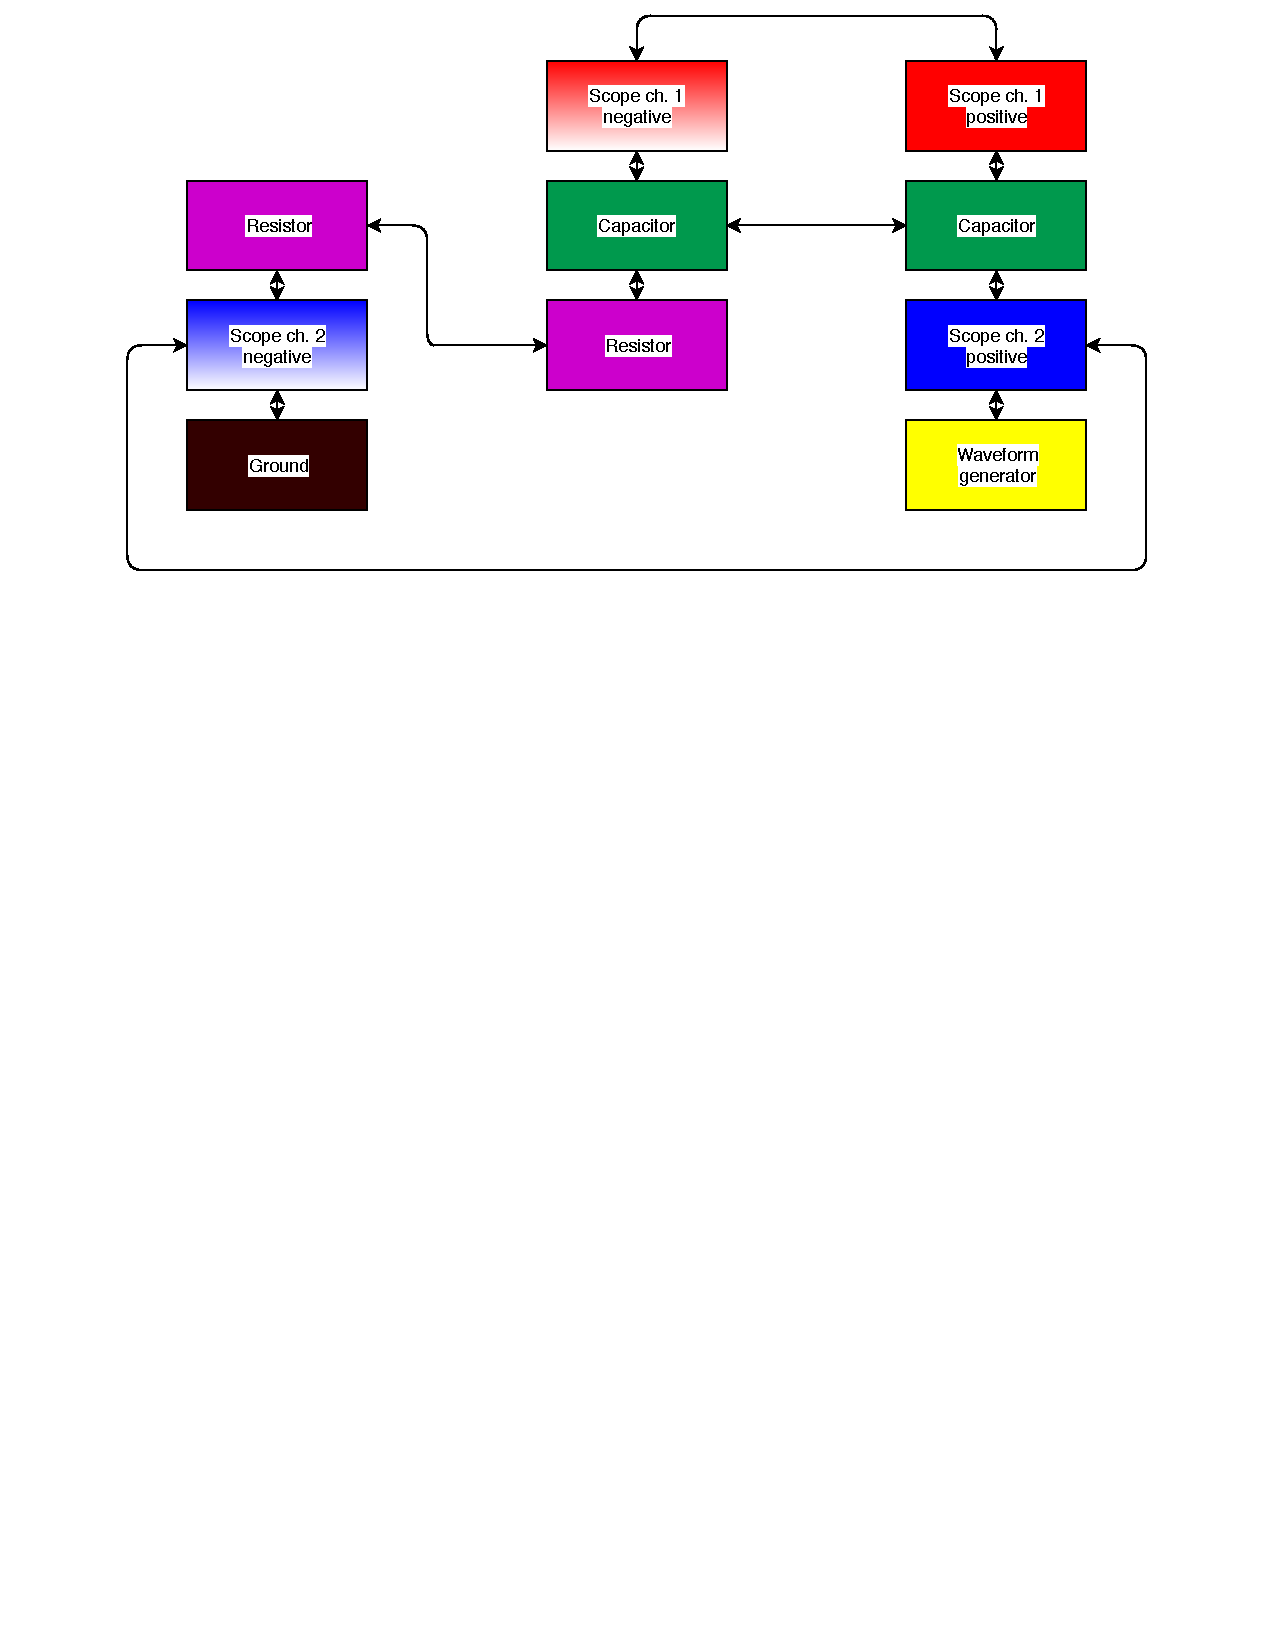
\includegraphics[clip, trim=0cm 18cm 0cm 0cm, scale=0.5]{fig/img/test_circuit_1}
	\caption{RC circuit}
\end{figure}
% Vær OBS på farvebeskrivelser af ledninger
This section uses the Analog Discovery 2 for setting up an RC circuit. The first step of the set-up is inserting a positive waveform generator (yellow) and a positive scope (blue) showing the waveforms. The waveform generator uses an AC step voltage. The current then passes through a resistor ($4.77 k\Omega$) and a capacitor ($97.61 nF$). Another scope is inserted to measure the charging and discharging of the capacitor. First, the current passes through a positive scope (orange), then the capacitor, and back through a negative scope (orange/white). Hypothetically, if the two scopes were switched, it would be measuring the inverse charging and discharging. Lastly, the current passes through a negative scope (blue/white) and into a negative waveform generator (yellow/white). Hereby, the circuit illustrated in REF is created with the same values as in the previous section. \\ \\
To get the test values compatible with the theoretical values, the frequency input has to be calculated as the hertz needed for the capacitor to charge and discharge. Therefore, the wave generator has to produce $214.6 Hz$  ($(2 \cdot 2.33 ms)^{-1} = 214.6 Hz$). \\
The data from the theoretical values and the test results can now be compared using python:
\begin{figure}[H]
\center
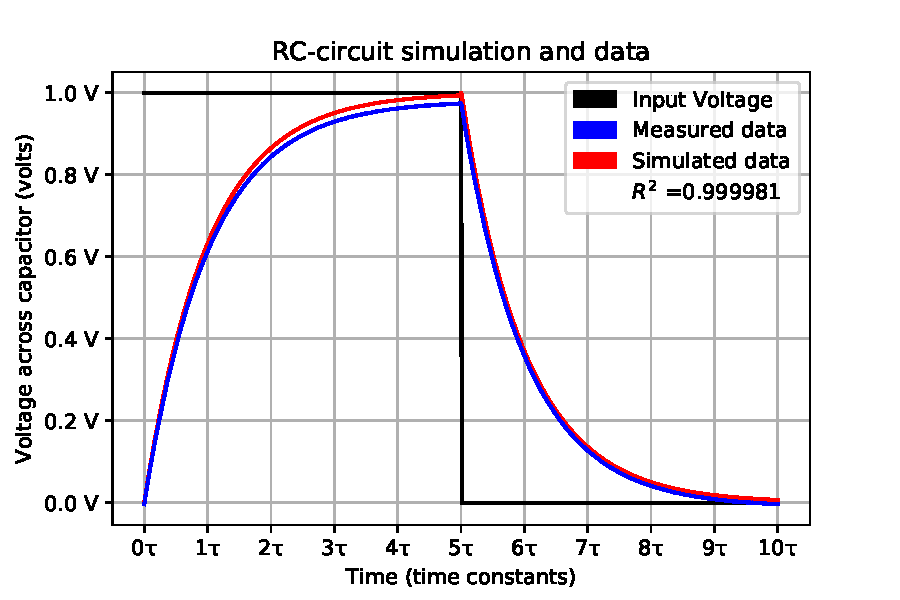
\includegraphics[scale=0.6]{fig/img/eks_1}
\end{figure}
As shown on the graph, the test results are very close to the calculated theoretical values. $R^2$ is almost equal to 1, which means that the two plots are almost identical.

